%\newcommand*{\SCRIPT}{}
\newcommand*{\BEAMER}{}

\ifdefined\SCRIPT
	\documentclass{article}
	\usepackage[a4paper, left=2.5cm, right=2cm, top=5.5cm, bottom=2.5cm]{geometry}
	\usepackage[noxcolor]{beamerarticle}
	\usepackage[ngerman]{babel}
	\usepackage[utf8]{inputenc}
	\usepackage{amsmath}
	\usepackage{amsthm}
	\usepackage{graphicx}
	\usepackage{pgfplots}
	\usepackage{tcolorbox}
	\usepackage{siunitx}
	\sisetup{locale = DE,
	per-mode=fraction}
	\usetikzlibrary{arrows,patterns}
	\usepackage{biblatex}
	\usepackage{xltabular}
	\addbibresource{Schallgeschwindigkeit.bib}
	\usepackage{scrlayer-scrpage}
	\pagestyle{scrheadings}
	\clearpairofpagestyles
	\ofoot{Seite \pagemark}
	\newcolumntype{C}[1]{>{\centering\arraybackslash}p{#1}}
	\DeclareNewLayer[%
	  background,% Hintergrundebene
	  width=\textwidth,% Größe und Position des Textbereichs
	  hoffset=2.5cm,
	  voffset=2.5cm,
	  align=tl,
	  contents={%
	  \sffamily
	    \setlength{\fboxsep}{2mm}% Abstand Box Text
	    \setlength{\fboxrule}{.5mm}% Dicke Linie
	    % vertikale Position korrigieren    
	    \vskip-\fboxsep\vskip-\fboxrule\vskip-\baselineskip
	    % horizontale Position korrigieren
	    \hspace{-\fboxsep}\hspace{-\fboxrule}%
	    \begin{tabularx}{\textwidth}{|>{\bfseries\Large}C{7cm}|X|X|}                                                       
	\hline
	\vspace{0em}
\includegraphics[scale=0.3]{logo2.png} & Name: & Datum: \\
	\hline
	
	\end{tabularx}
	    %\makebox[\layerwidth][l]{%
	    %  \fbox{\rule{0pt}{\layerheight}\rule{\layerwidth}{0pt}}% Rahmen
	    %}%
	  }
	]{frame}
	\AddLayersToPageStyle{@everystyle@}{frame}
\fi

\ifdefined\BEAMER
	\documentclass{beamer}
	\usepackage[ngerman]{babel}
	\usepackage[utf8]{inputenc}
	\usepackage{amsmath}
	\usepackage{amsthm}
	\usepackage{graphicx}
	\usepackage{pgfplots}
	\usepackage{tcolorbox}
	\usepackage{siunitx}
	\sisetup{locale = DE,
	per-mode=fraction}
	\usetikzlibrary{arrows,patterns}
	% Lade Beamer Stile
	\usetheme{Rochester}
	\usecolortheme{crane}
	\usepackage{beamerthemesplit}
\fi

\title{5. Unterrichtseinheit zur Dynamik}
\subtitle{Energieerhaltungssatz}
\author{Heiko Schröter}
\date{\today}

\setbeamertemplate{enumerate item}{\alph{enumi})}

\begin{document}

\frame{\titlepage}

\frame
{
  \frametitle{Ziele für die heutige Unterrichtseinheit}
  \textbf{Energieerhaltungssatz}
  \begin{itemize}
	\item Was besagt der Energieerhaltungssatz?
	\item Beispiel (In)elastischer Stoß
	\item Beispiel Pendel
	\item Beispielaufgabe
	\item Übungsaufgaben
	\item Überblick Energie, Kraft, Arbeit, Leistung, Potential, Feld
  \end{itemize}
}

\frame
{
  \frametitle{Energieerhaltungssatz}
\begin{block}{Beschreibung}
Die Summe der Energien am Ende eines technischen Vorgangs ist genauso groß wie die Summe der Energien am Anfang und während des technischen Vorgangs zugeführten und abzüglich der abgeführten Energien.
\begin{align*}
W_{Ende}=W_{Anfang}+W_{zu}-W_{ab}
\end{align*}
\end{block}
Innerhalb eines Systems kann Energie beliebig oft zwischen verschiedenen Energieformen hin und her gewandelt werden, die Summe aller Energien bleibt jedoch unverändert.
}

\frame
{
  \frametitle{Beispiel Fadenpendel}
      \begin{figure}
	    \begin{tikzpicture}
  \begin{scope}[scale=0.3]
  \begin{footnotesize}
  	\draw[thin] (0,4) -- (0,10) node[midway, right] {$y$};
  	%\draw[latex-,thin,blue] (0,0.75) -- (0,4);
  	\draw[thin] (-8,10) -- (8,10);
   	\fill[black] (0,10) circle (0.1);
   	\fill[pattern=north east lines, very thin] (-8,10) -- (8,10) -- (8,10.5) -- (-8,10.5) -- cycle;
   	\draw [shift={(0.,10.)},thin,red,dashed]  plot[domain=3.7850937623830774:5.639684198386302,variable=\t]({1.*10.*cos(\t r)+0.*10.*sin(\t r)},{0.*10.*cos(\t r)+1.*10.*sin(\t r)});
   	\draw[thin] (0,10) -- (-8,4) node[midway, above] {$l$};
   	\draw[thin] (0,10) -- (8,4) node[midway, above] {$l$};
   	\draw[thin] (-8,4) -- (0,4) node[midway, below] {$S$};
   	\draw[thin] (0,4) -- (8,4) node[midway, below] {$S$};
	\shadedraw[inner color=black!10!white,outer color=black!30!white, draw=black] (-8,4) circle (1) node {$B$};
	\shadedraw[inner color=black!10!white,outer color=black!30!white, draw=black] (8,4) node {$C$} circle (1);
	\shadedraw[inner color=black!10!white,outer color=black!30!white, draw=black] (0,0) node {$A$} circle (1);
	\draw [shift={(0,10)},thin,green] (-90:2) arc  (-90.:-36.86989764584402:2) node[near start, above] {$\varphi$};
	\draw [shift={(0,10)},thin,green,]  (-143.13010235415598:2) arc (-143.13010235415598:-90:2)node[near end, above]{$\varphi$};
	\draw[latex-latex,thin,blue] (0,0) -- (0,4) node[midway, right] {$h$};
	\node at (-8,0) {\begin{tabular}{l}
    $E_{pot}=max$ \\ 
    $E_{kin}=0$
	\end{tabular}};
	\node at (8,0) {\begin{tabular}{l}
    $E_{pot}=max$ \\ 
    $E_{kin}=0$
	\end{tabular}};
	\node at (0,-2) {\begin{tabular}{l}
    $E_{kin}=max$ \\ 
    $E_{pot}=0$
	\end{tabular}};
  \end{footnotesize}
  \end{scope}
  \end{tikzpicture}
	  \vspace{-3mm}
	  \caption{Energieumwandlung}
   \end{figure}
  % Kinetische Energie wird in potentielle Energie und zurück gewandelt.
  \begin{block}{}
	\begin{align*}
	E_{kin}=\frac{1}{2}mv^2\quad
	E_{pot}=m\cdot g\cdot \Delta h
	\end{align*}
  \end{block}
}


\frame
{
  \frametitle{Beispiel Fadenpendel}
  \begin{block}{Energieerhaltung}
  Ohne Reibung, ohne Luftwiederstand
	\begin{align*}
	E_{kin}=E_{pot}\quad\Rightarrow\quad \frac{1}{2}mv^2\quad=m\cdot g\cdot \Delta h
	\end{align*}
  \end{block}
}

\frame
{
  \frametitle{Beispielaufgabe Fadenpendel}
\uncover<1->
{
  Ein Pendel (Masse \SI{100}{\gram}, Länge \SI{1.5}{\meter}) wird um \SI{15}{\centi\meter} ausgelenkt. Welche Geschwindigkeit hat es beim Durchqueren des Gleichgewichtspunktes?\\
}
\uncover<2->
{
\textbf{Lösung:}	\begin{align*}
	E_{kin}&=E_{pot}\quad\Rightarrow\quad \frac{1}{2}mv^2\quad=m\cdot g\cdot \Delta h\\
	\Delta h&=l-y\Rightarrow y=\sqrt{l^2-s^2}\Rightarrow \Delta h=l-\sqrt{l^2-s^2}\\
	v&=\sqrt{2\cdot g\cdot \Delta h}=\sqrt{2\cdot g \cdot \left( l-\sqrt{l^2-s^2}\right)}\\
	v&=\sqrt{2\cdot \SI{9,81}{\meter\square\second} \cdot \left( (\SI{1.5}{\meter})-\sqrt{(\SI{1.5}{\meter})^2-(\SI{0.15}{\meter})^2}\right)}\\
	v&=\SI{0,384}{\meter\per\second}=\SI{38,4}{\centi\meter\per\second}
	\end{align*}
}
}

\frame
{
  \frametitle{Beispiel realer Stoß}
  \begin{block}{Energiebilanz}
	\begin{align*}
	\text{verlustfreier Stoß}
	\quad W_1&=W_2\\
	\text{realer Stoß}
	\quad W_1&=W_2+\Delta W
	\end{align*}
	Die Endgeschwindigkeiten beim realen Stoß sind kleiner als beim vollkommen elastischen Stoß.
  \end{block}
}

\frame
{
  \frametitle{Energieumwandlung beim realen Stoß}
  \begin{tikzpicture}
  \begin{scope}[yscale=50, xscale=5]
    %\draw[very thin,color=gray,xstep=0.1, ystep=0.01] (0,0) grid (1.05,0.095);
    \draw[->] (0,0) -- (1.1,0) node[right] {$t$};
    \draw[->] (0,0) -- (0,0.1) node[above] {$h$};
    \draw[domain=0:0.298] plot ({\x},{-(\x-0.298)*(\x+0.298)});
    \node[left] () at (0,0.088804) {$h_0=\SI{17,2}{\centi\meter}$};
    \draw[domain=0.298:0.524] plot ({\x},{-4*(\x-0.298)*(\x-0.524)});
    \draw[domain=0.524:0.707] plot ({\x},{-4*(\x-0.707)*(\x-0.524)});
    \draw[domain=0.707:0.859] plot ({\x},{-4*(\x-0.707)*(\x-0.859)});
    \draw[domain=0.859:0.988] plot ({\x},{-4*(\x-0.988)*(\x-0.859)});
    %\draw (0,0.088804) -- (,0.088804);
    \draw[dotted, very thin] (0,2*0.025538) node[left] {$h_1=\SI{10,9}{\centi\meter}$} -- (0.411,2*0.025538);
    \draw[dotted, very thin] (0,2*0.016745) node[left] {$h_2=\SI{6,2}{\centi\meter}$} -- (0.6155,2*0.016745);
    \draw[dotted, very thin] (0,2*0.011552) node[left] {$h_3=\SI{4,1}{\centi\meter}$} -- (0.783,2*0.011552);
    \draw[dotted, very thin] (0,2*0.008321) node[left] {$h_4=\SI{2,8}{\centi\meter}$} -- (0.9235,2*0.008321);
    \node[below] () at (0.149,-0.002) {$\Delta t_1$};
    \node[below] () at (0.411,-0.002) {$\Delta t_2$};
    \node[below] () at (0.6155,-0.002) {$\Delta t_3$};
    \node[below] () at (0.783,-0.002) {$\cdots$};
    \filldraw[fill=yellow!60!, draw=black!40!yellow, thick] (0,0.088804) ellipse (0.02cm and 0.002cm);
    \filldraw[fill=white, draw=black!40!yellow, thin] (0.298,0) ellipse (0.02cm and 0.002cm);
  \end{scope}
  \end{tikzpicture}
}

\frame
{
\uncover<1->
{
  \frametitle{Beispielaufgabe Stoß}
Mit welcher Geschwindigkeit schlägt die Kugel beim ersten Aufschlag auf dem Boden auf, wenn die Kugel aus einer maximalen Höhe von \SI{17,2}{\centi\meter} fällt? Welche Geschwindigkeit hat sie \SI{10}{\centi\meter} über dem Boden?\\
}
\uncover<2->
{
\textbf{Lösung:}	
	\begin{align*}
	E_{pot}&=E_{kin}\quad\Rightarrow\quad m\cdot g\cdot h=\frac{1}{2}mv^2\\
	v&=\sqrt{2\cdot g\cdot h}=\sqrt{2\cdot \SI{9,81}{\meter\per\square\second}\cdot \SI{0,172}{\meter}}\\
	&=\SI{1,84}{\meter\per\second}=\SI{6,61}{\kilo\meter\per\hour}\\
	v_x&=\sqrt{2\cdot g\cdot\Delta h}=\sqrt{2\cdot \SI{9,81}{\meter\per\square\second}\cdot\SI{0,072}{\meter}}\\
	&=\SI{1,19}{\meter\per\second}=\SI{4,28}{\kilo\meter\per\hour}
	\end{align*}
}
}

\frame
{
  \frametitle{Beispielaufgabe Feder}
Eine Feder mit der Federkonstante $D=\SI{20}{\newton\centi\meter}$ ist um \SI{4}{\centi\meter} gestaucht.
\begin{enumerate}
\item Wie viel Energie ist in der Feder gespeichert? Wie hoch könnte man einen Liter Wasser mit dieser Energie heben?
\item Die Feder wird benutzt, um eine Metallkugel der Masse $m=\SI{30}{\gram}$ senkrecht nach oben zu schießen. Welche Höhe erreicht die Kugel dabei?
\item Die Kugel fällt nun wieder nach unten. Mit welcher Geschwindigkeit schlägt sie wieder auf dem Boden auf? Welche Geschwindigkeit hat sie \SI{5}{\meter} über dem Boden?
\end{enumerate}
}
\frame[allowframebreaks]
{
\textbf{Lösung:}	
\begin{enumerate}
\item 
	\begin{align*}
	E_{sp}&=\frac{1}{2}\cdot D \cdot s^2=\frac{1}{2}\cdot \SI{20}{\newton\centi\meter} \cdot (\SI{4}{\centi\meter})^2=\SI{160}{\newton\centi\meter}=\SI{1,6}{\newton\meter}\\
	E_{pot}&=m\cdot g\cdot h=\SI{1,6}{\newton\meter}=\SI{1}{\kilo\gram}\cdot\SI{9,81}{\meter\per\square\second}\cdot h\\
	\Rightarrow h&=\dfrac{\SI{1,6}{\newton\meter}}{\SI{1}{\kilo\gram}\cdot\SI{9,81}{\meter\per\square\second}}=\SI{0,163}{\meter}
	\end{align*}
	In der Feder sind \SI{1,6}{\newton\meter} gespeichert. Mit dieser Energie könnte man einen Liter Wasser um \SI{16,3}{\centi\meter} anheben.
\item 
	\begin{align*}
	E_{sp}&=E_{pot}\Rightarrow \SI{1,6}{\newton\meter}=m\cdot g\cdot h\Rightarrow \\
	h&=\dfrac{\SI{1,6}{\newton\meter}}{\SI{0,03}{\kilo\gram}\cdot\SI{9,81}{\meter\per\square\second}}=\SI{5,44}{\meter}
	\end{align*}
	Die Kugel erreicht eine Höhe von \SI{5,44}{\meter}.\newpage
\item 
	\begin{align*}
	E_{pot}&=E_{kin}\Rightarrow m\cdot g\cdot h=\frac{1}{2}\cdot m \cdot v^2\Rightarrow v=\sqrt{2\cdot g\cdot h}\\
	v&=\sqrt{2\cdot \SI{9,81}{\meter\per\square\second}\cdot \SI{5,44}{\meter}}=\SI{10,3}{\meter\per\second}=\SI{37,2}{\kilo\meter\per\hour}\\
	v_x&=\sqrt{2\cdot g\cdot \Delta h}=\sqrt{2\cdot \SI{9,81}{\meter\per\square\second}\cdot (\SI{5,44}{\meter}-\SI{5}{\meter})}\\
	&=\sqrt{2\cdot \SI{9,81}{\meter\per\square\second}\cdot \SI{0,44}{\meter}}=\SI{2,94}{\meter\per\second}=\SI{10,6}{\kilo\meter\per\hour}
	\end{align*}
	Die Kugel schlägt mit \SI{37,2}{\kilo\meter\per\hour} auf dem Boden auf, \SI{5}{\meter} über dem Boden hat sie eine Geschwindigkeit von \SI{10,6}{\kilo\meter\per\hour}.
\end{enumerate}
}

\frame
{
  \frametitle{Überblick über Begriffe der Mechanik}
\begin{block}{Beschreibung}
\vspace{0.5cm}
% \usepackage{array} is required
\begin{tabular}{|>{\centering\arraybackslash}p{3cm}|>{\centering\arraybackslash}p{3cm}|>{\centering\arraybackslash}p{3cm}|}
\hline
\rule[-1ex]{0pt}{2.5ex} Energie & Kraft & Arbeit \\
\hline 
\rule[-1ex]{0pt}{2.5ex} Leistung & Potential & Feld \\ 
\hline 
\end{tabular}
\vspace{0.5cm}
\end{block}
Am Beispiel der schiefen Ebene.
}

\frame
{
  \frametitle{Energie}
\begin{block}{Beschreibung}
Unter Energie versteht man gespeicherte Arbeit, d.h. Fähigkeit eines Systems, Arbeit zu verrichten. Energie kann zwischen verschiedenen Energieformen hin- und her gewandelt werden, aber die Gesamtenergie bleibt dabei erhalten (Energieerhaltungssatz).
\end{block}
Die SI-Einheit der Energie $E$ ist:
$[E]=\SI{1}{\newton\meter}=\SI{1}{\joule}=\SI{1}{\kilo\gram\square\meter\per\square\second}$
      \begin{figure}
	  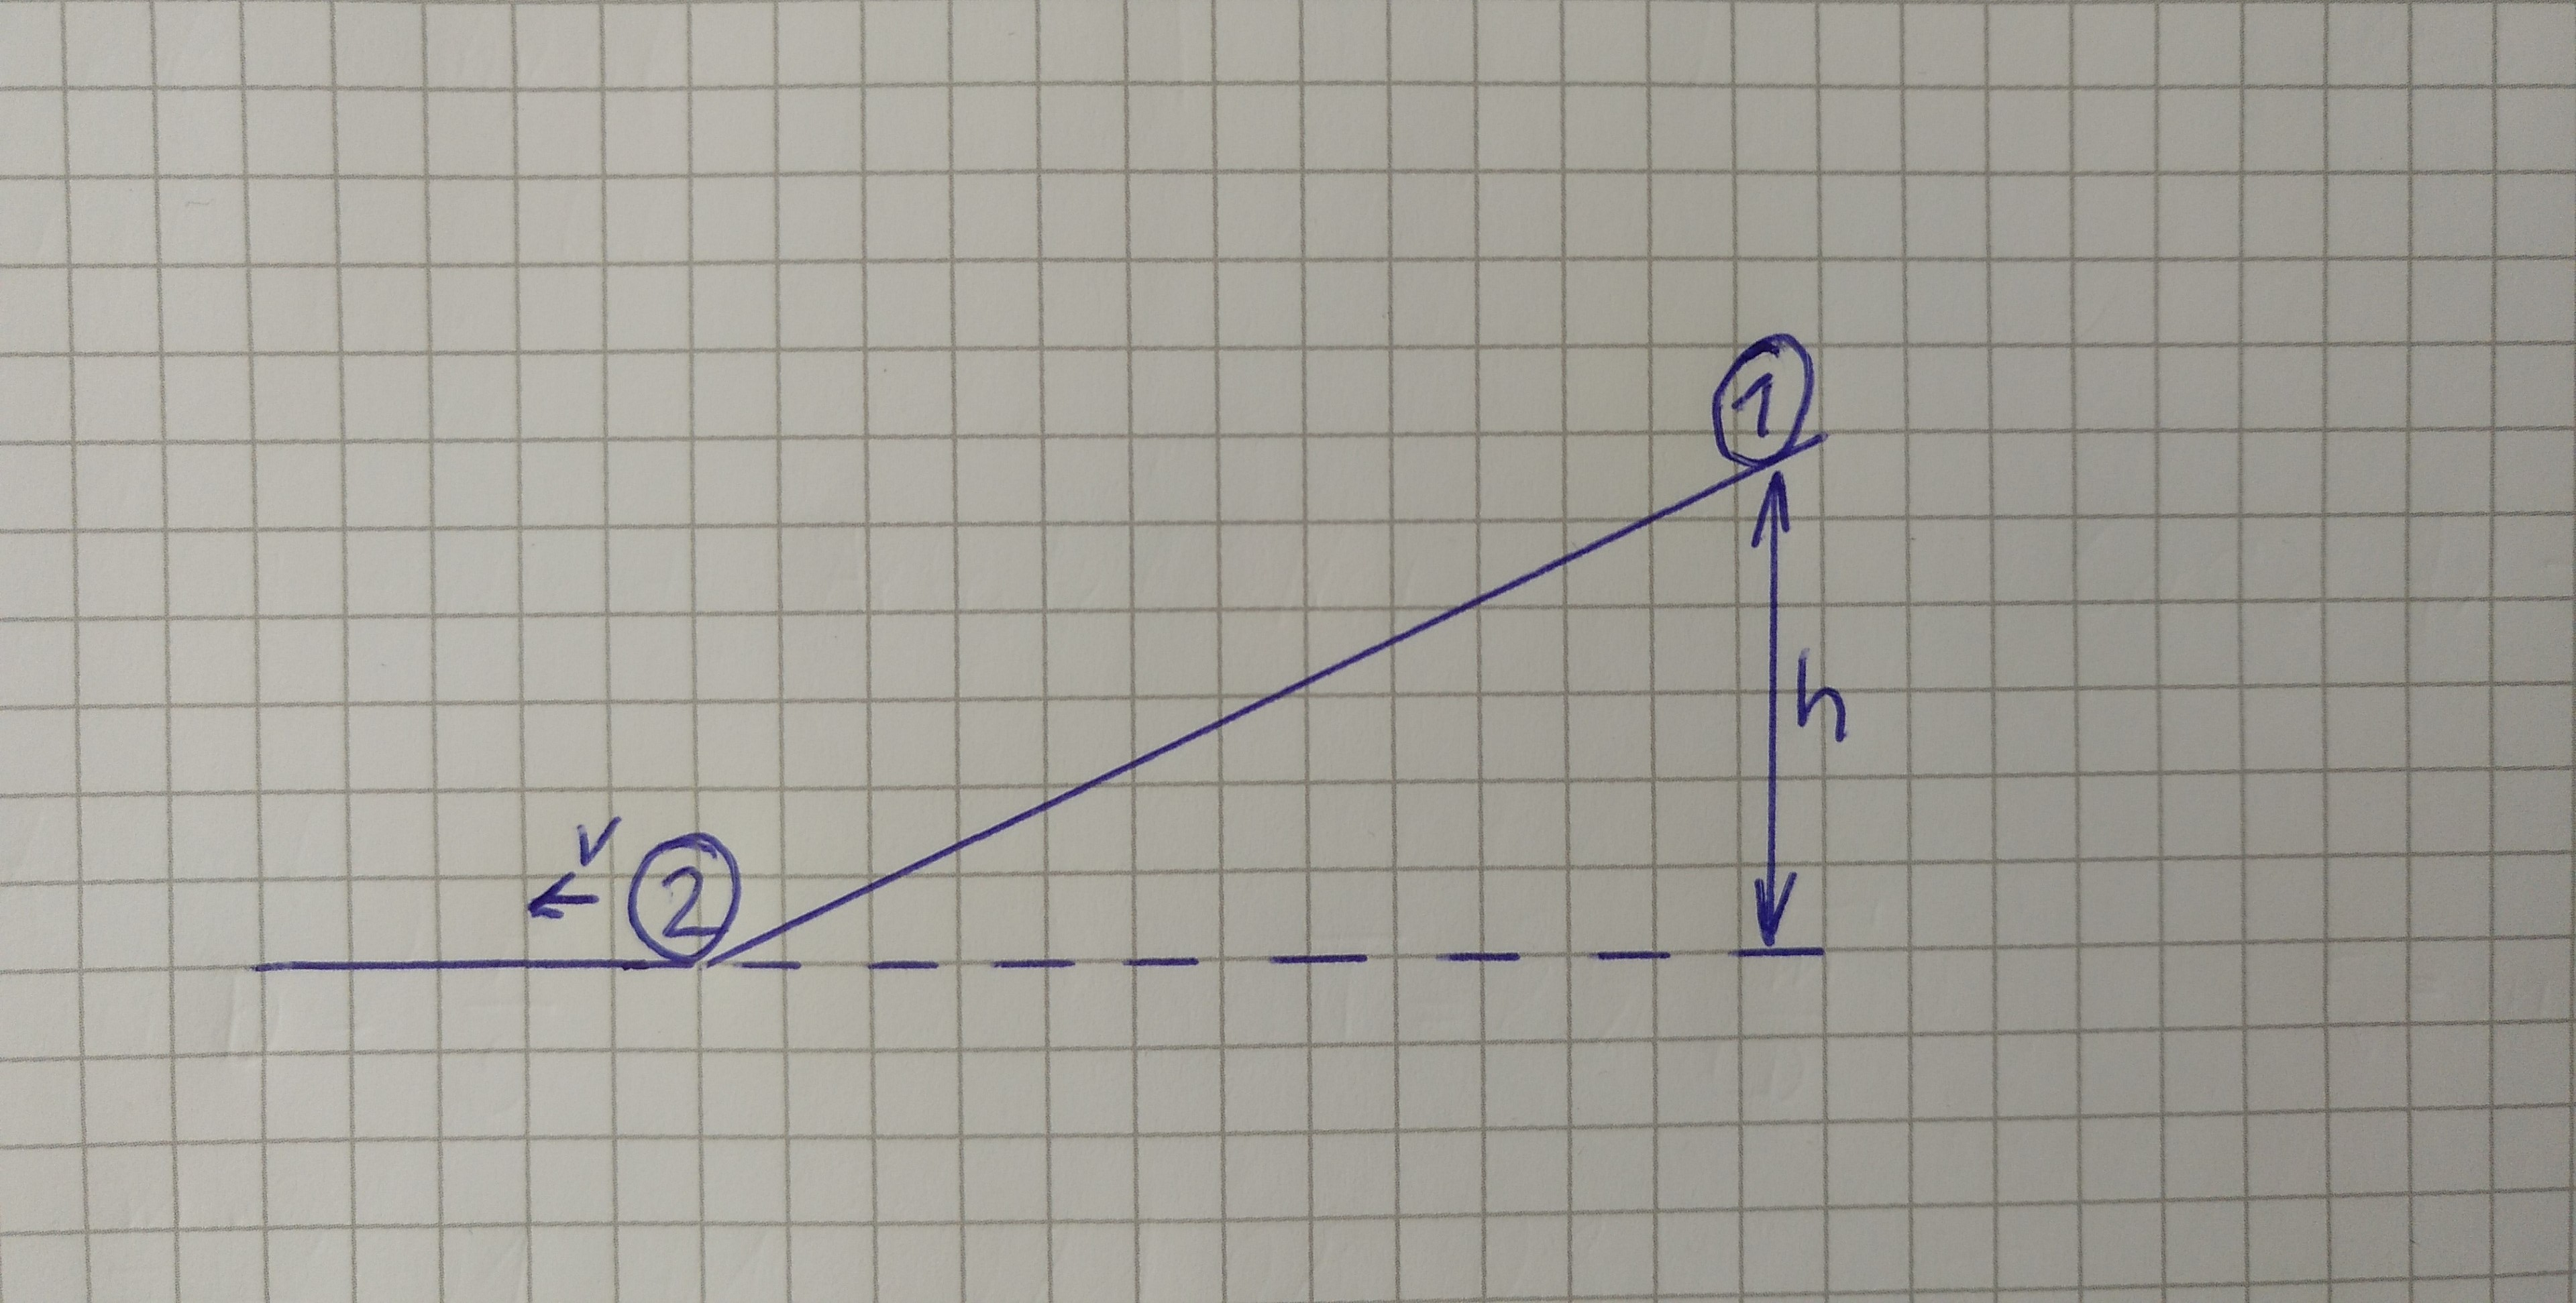
\includegraphics[width=0.8\textwidth]{Energie_1}
	  \vspace{-3mm}
	  \caption{Energie an der schiefen Ebene}
   \end{figure}
}

\frame
{
  \frametitle{Kraft}
\begin{block}{Beschreibung}
Eine Kraft ist durch ihre Größe (Stärke), ihre Richtung und ihren Angriffspunkt eindeutig bestimmt. Sie kann Körper verformen oder beschleunigen.
\end{block}
Die SI-Einheit der Kraft $F$ ist:
$[F]=\SI{1}{\newton}=\SI{1}{\kilo\gram\meter\per\square\second}$
      \begin{figure}
	  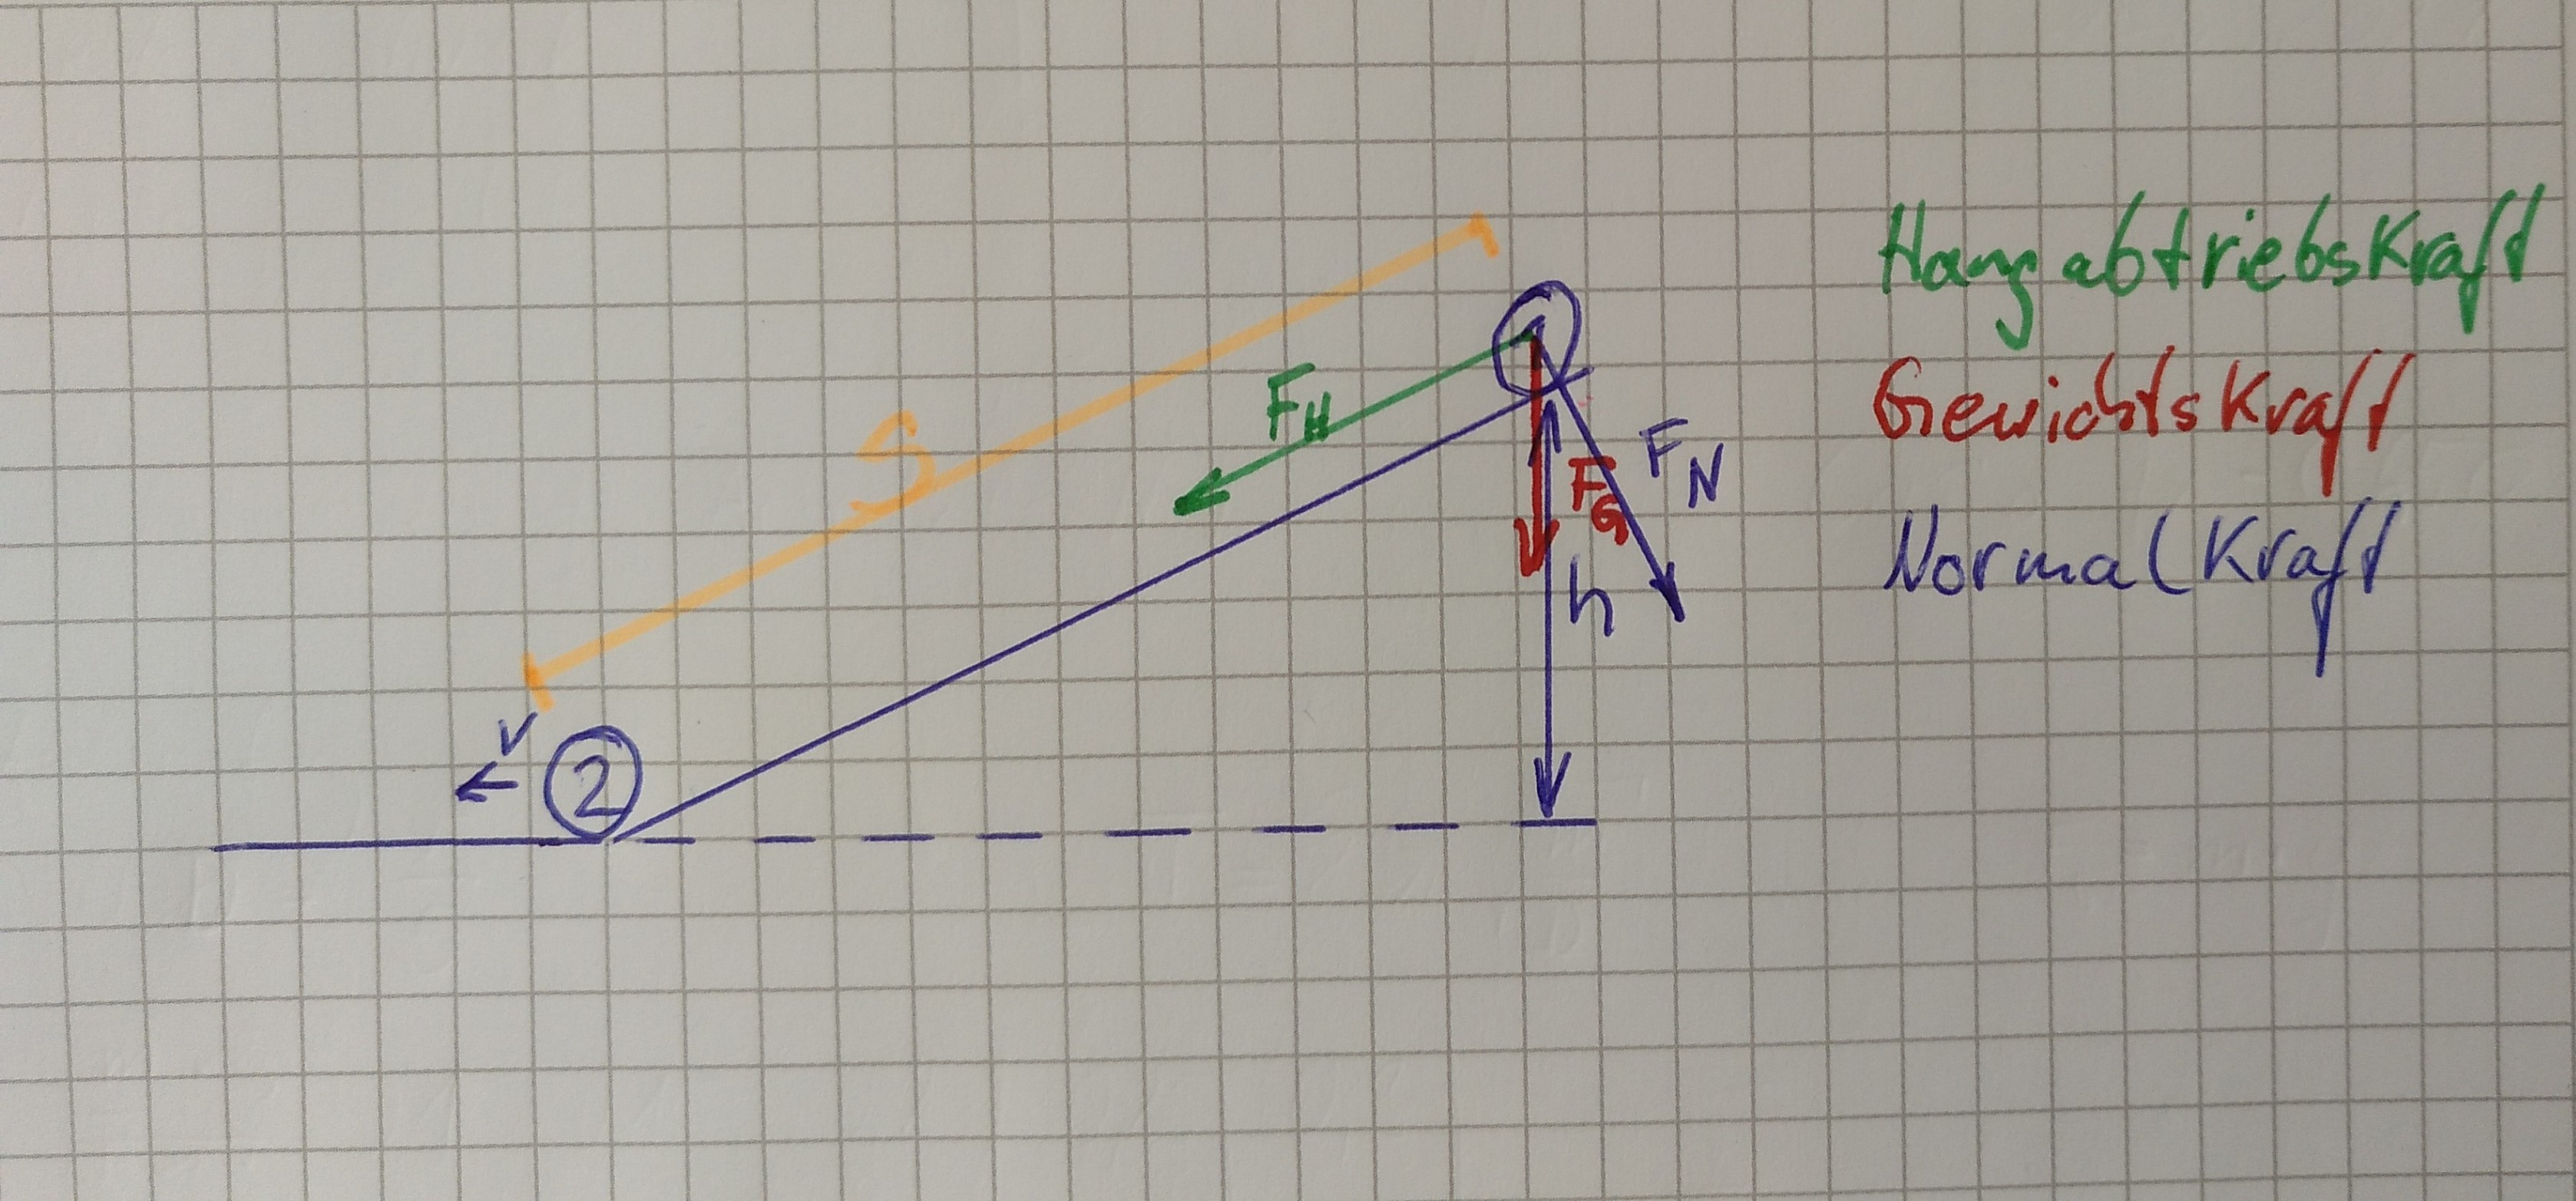
\includegraphics[width=0.8\textwidth]{Kraft}
	  \vspace{-3mm}
	  \caption{Kräfte an der schiefen Ebene}
   \end{figure}
     Wirkt die Kraft entlang eines Weges, so kann sie Energie übertragen bzw. Arbeit verrichten.
}

\frame
{
  \frametitle{Arbeit}
\begin{block}{Beschreibung}
Arbeit ist das Produkt aus der wirkenden Kraft $F$ und dem zurückgelegten Weg $s$ des bewegten Körpers. Durch Arbeit kann Energie in eine andere Form gewandelt werden.
\end{block}
Die SI-Einheit der Arbeit $W$ ist:
$[W]=\SI{1}{\newton\meter}=\SI{1}{\kilo\gram\square\meter\per\square\second}=\SI{1}{\joule}$
      \begin{figure}
	  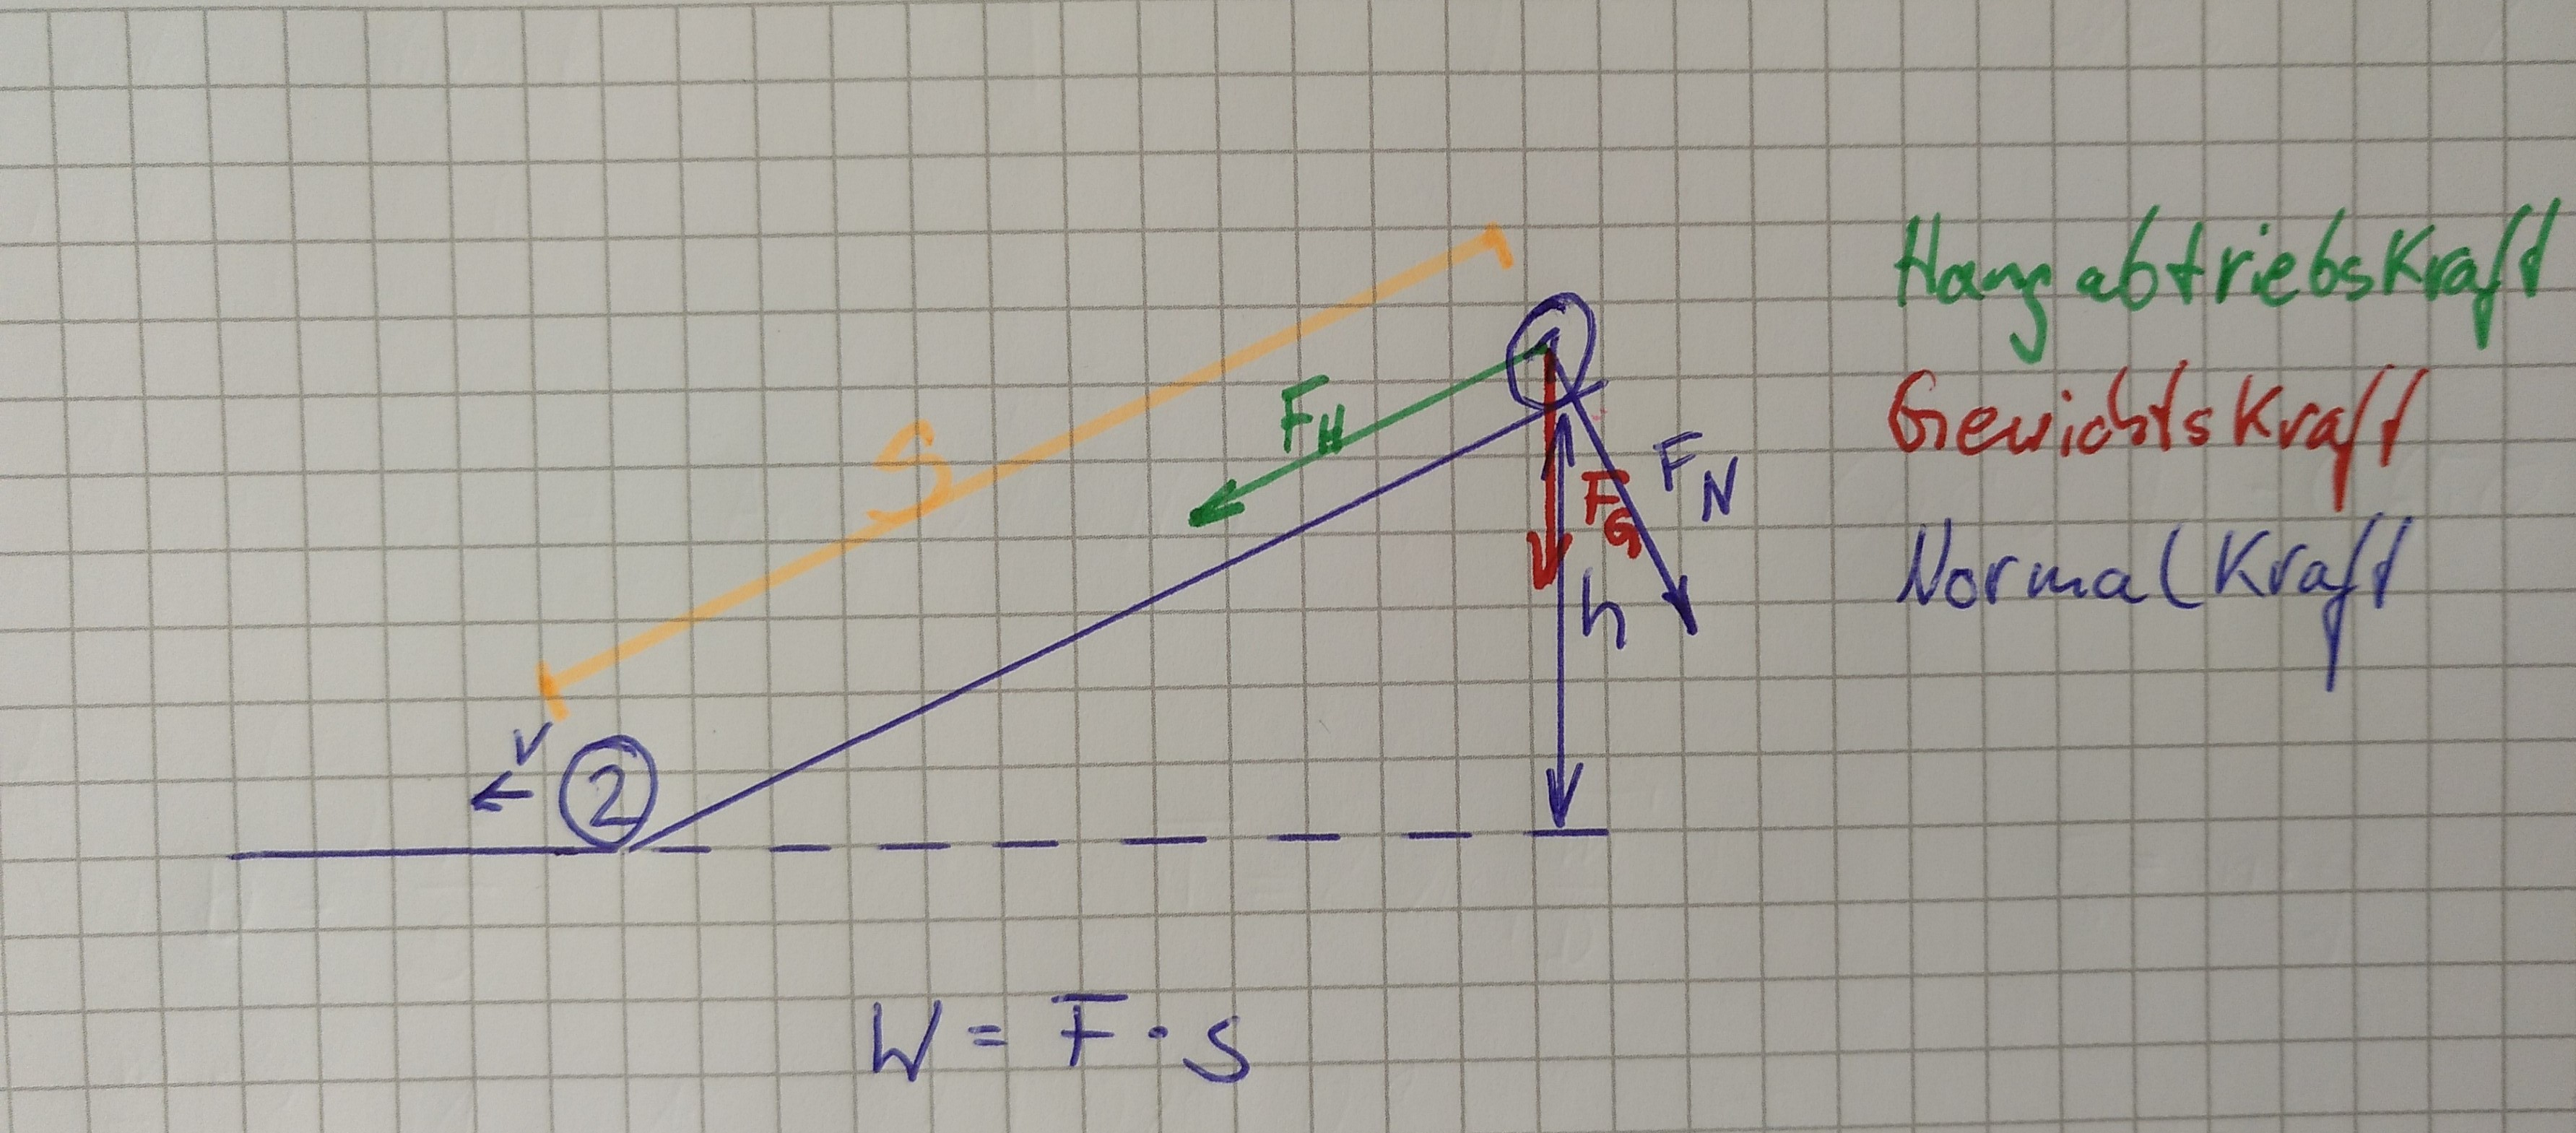
\includegraphics[width=0.8\textwidth]{Arbeit_1}
	  \vspace{-3mm}
	  \caption{Arbeit an der schiefen Ebene}
   \end{figure}
}

\frame
{
  \frametitle{Leistung}
\begin{block}{Beschreibung}
Die mechanische Leistung ist gleich dem Quotienten aus der mechanischen Arbeit und der für die Verrichtung dieser Arbeit erforderlichen Zeit. Sie gibt an, in welchem Maß ein System Arbeit verrichten kann.
\end{block}
SI-Einheit der Leistung $P$:
$[P]=\SI{1}{\newton\meter\per\second}=\SI{1}{\joule\per\second}=\SI{1}{\kilo\gram\square\meter\per\cubic\second}=\SI{1}{\watt}$
      \begin{figure}
	  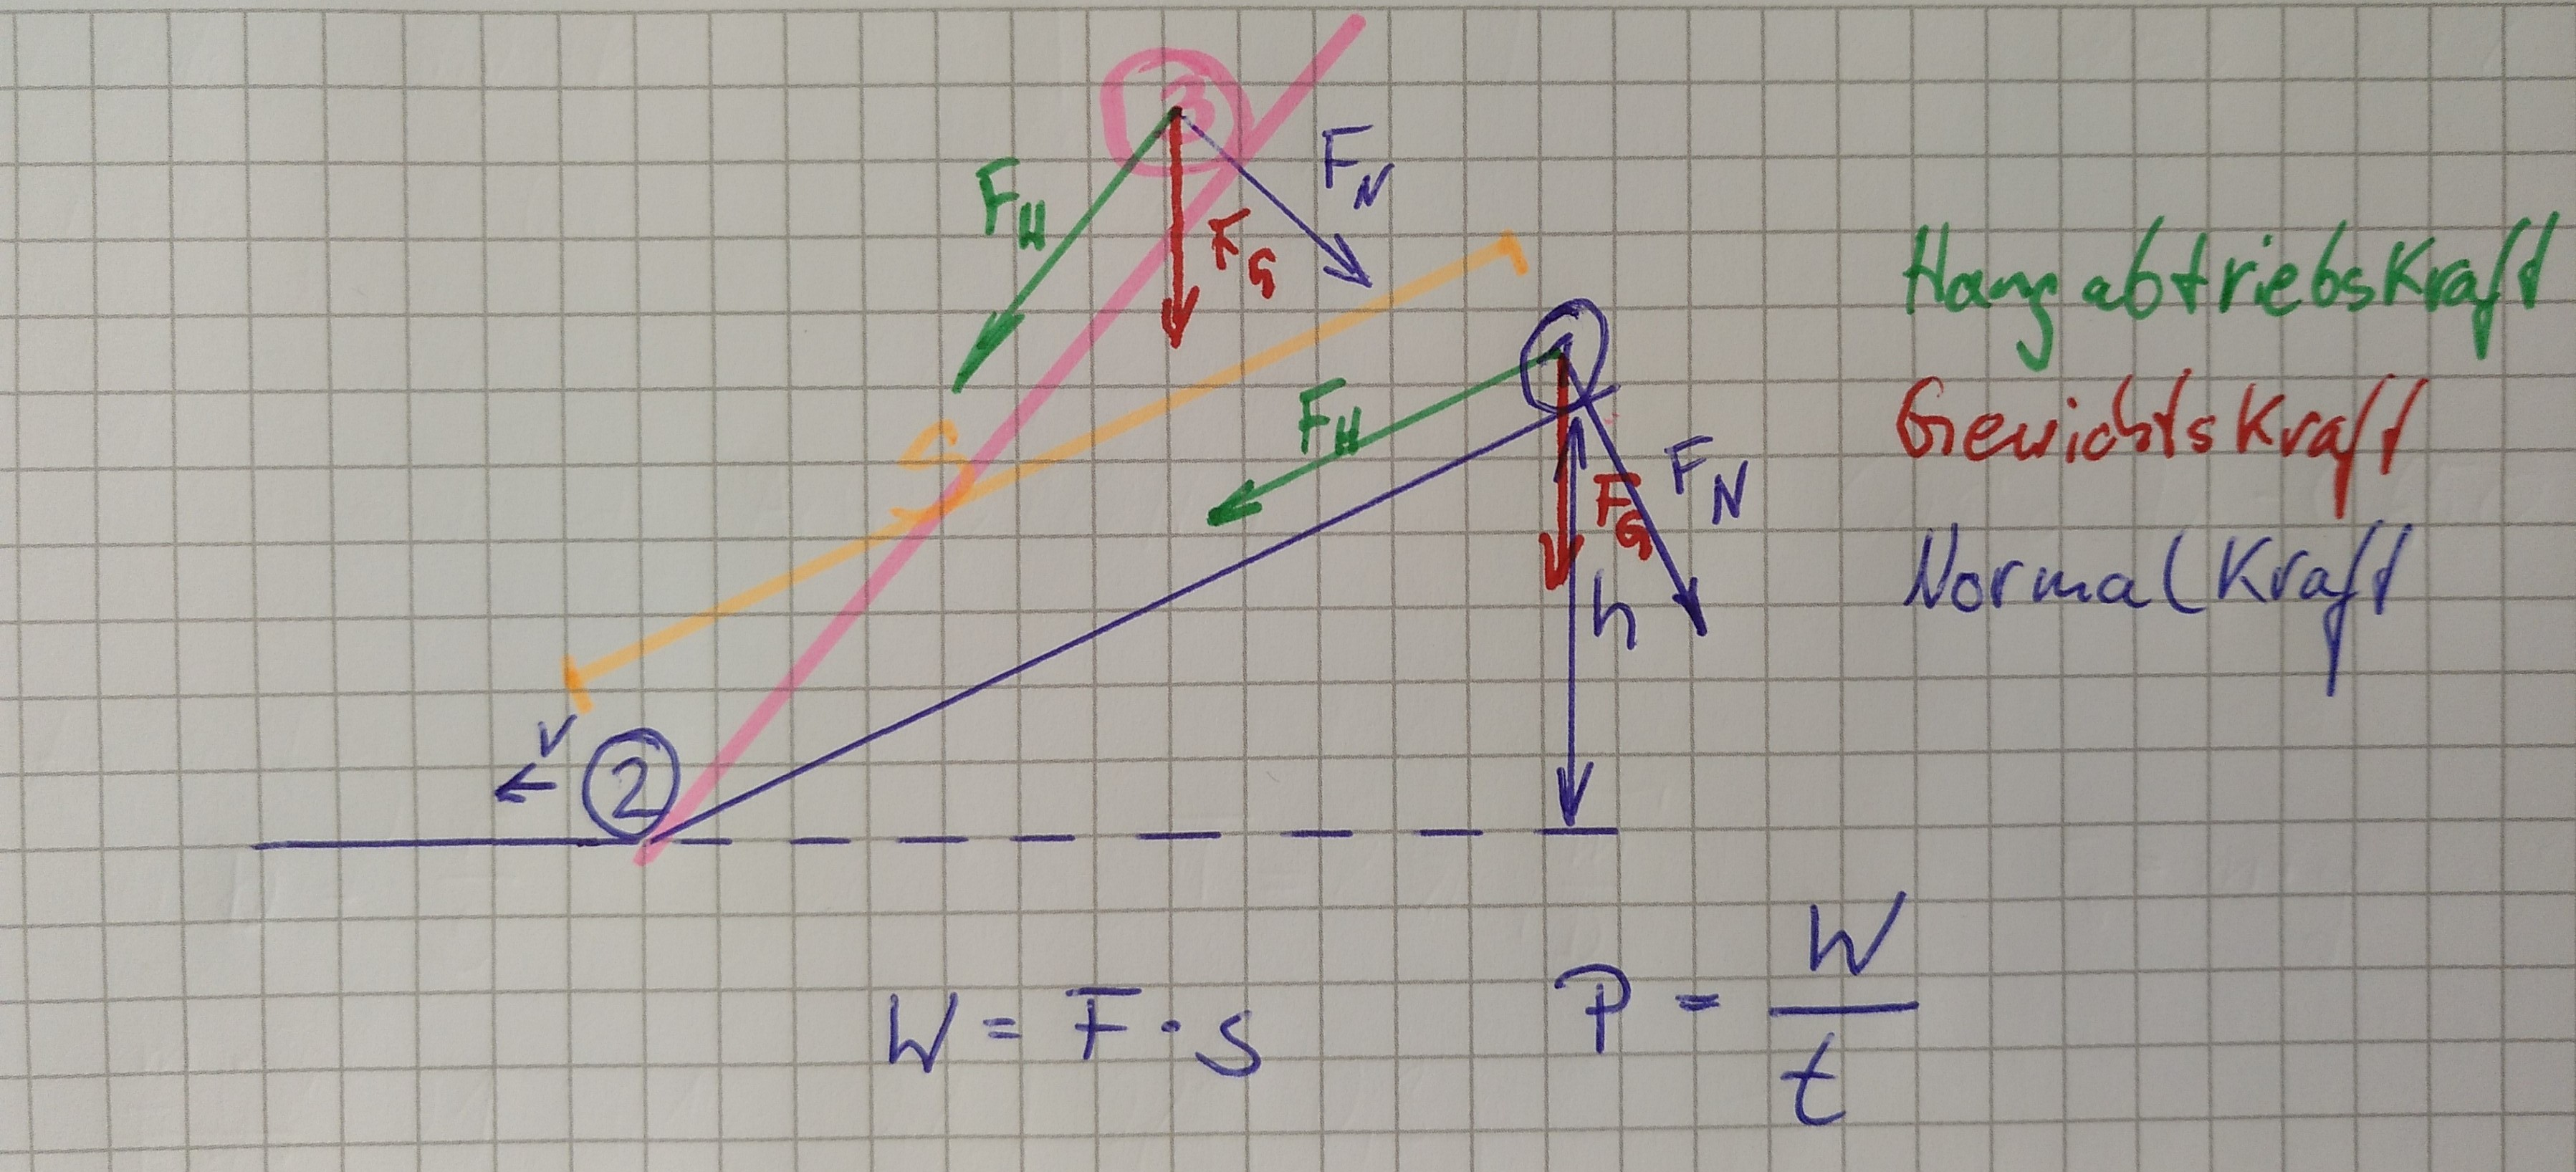
\includegraphics[width=0.6\textwidth]{Leistung}
	  \vspace{-3mm}
	  \caption{Leistung an der schiefen Ebene}
   \end{figure}
   Je mehr Energie ein System pro Sekunde umwandeln kann, desto größer ist seine Leistung.
}

\frame
{
  \frametitle{Potential}
\begin{block}{Beschreibung}
Das Potential, das ein Körper in einem Feld hat, beschreibt, wie viel Arbeit das Feld an ihm verrichten kann. Das Potential hängt vom gewählten Bezugspunkt ab.
\end{block}
      \begin{figure}
	  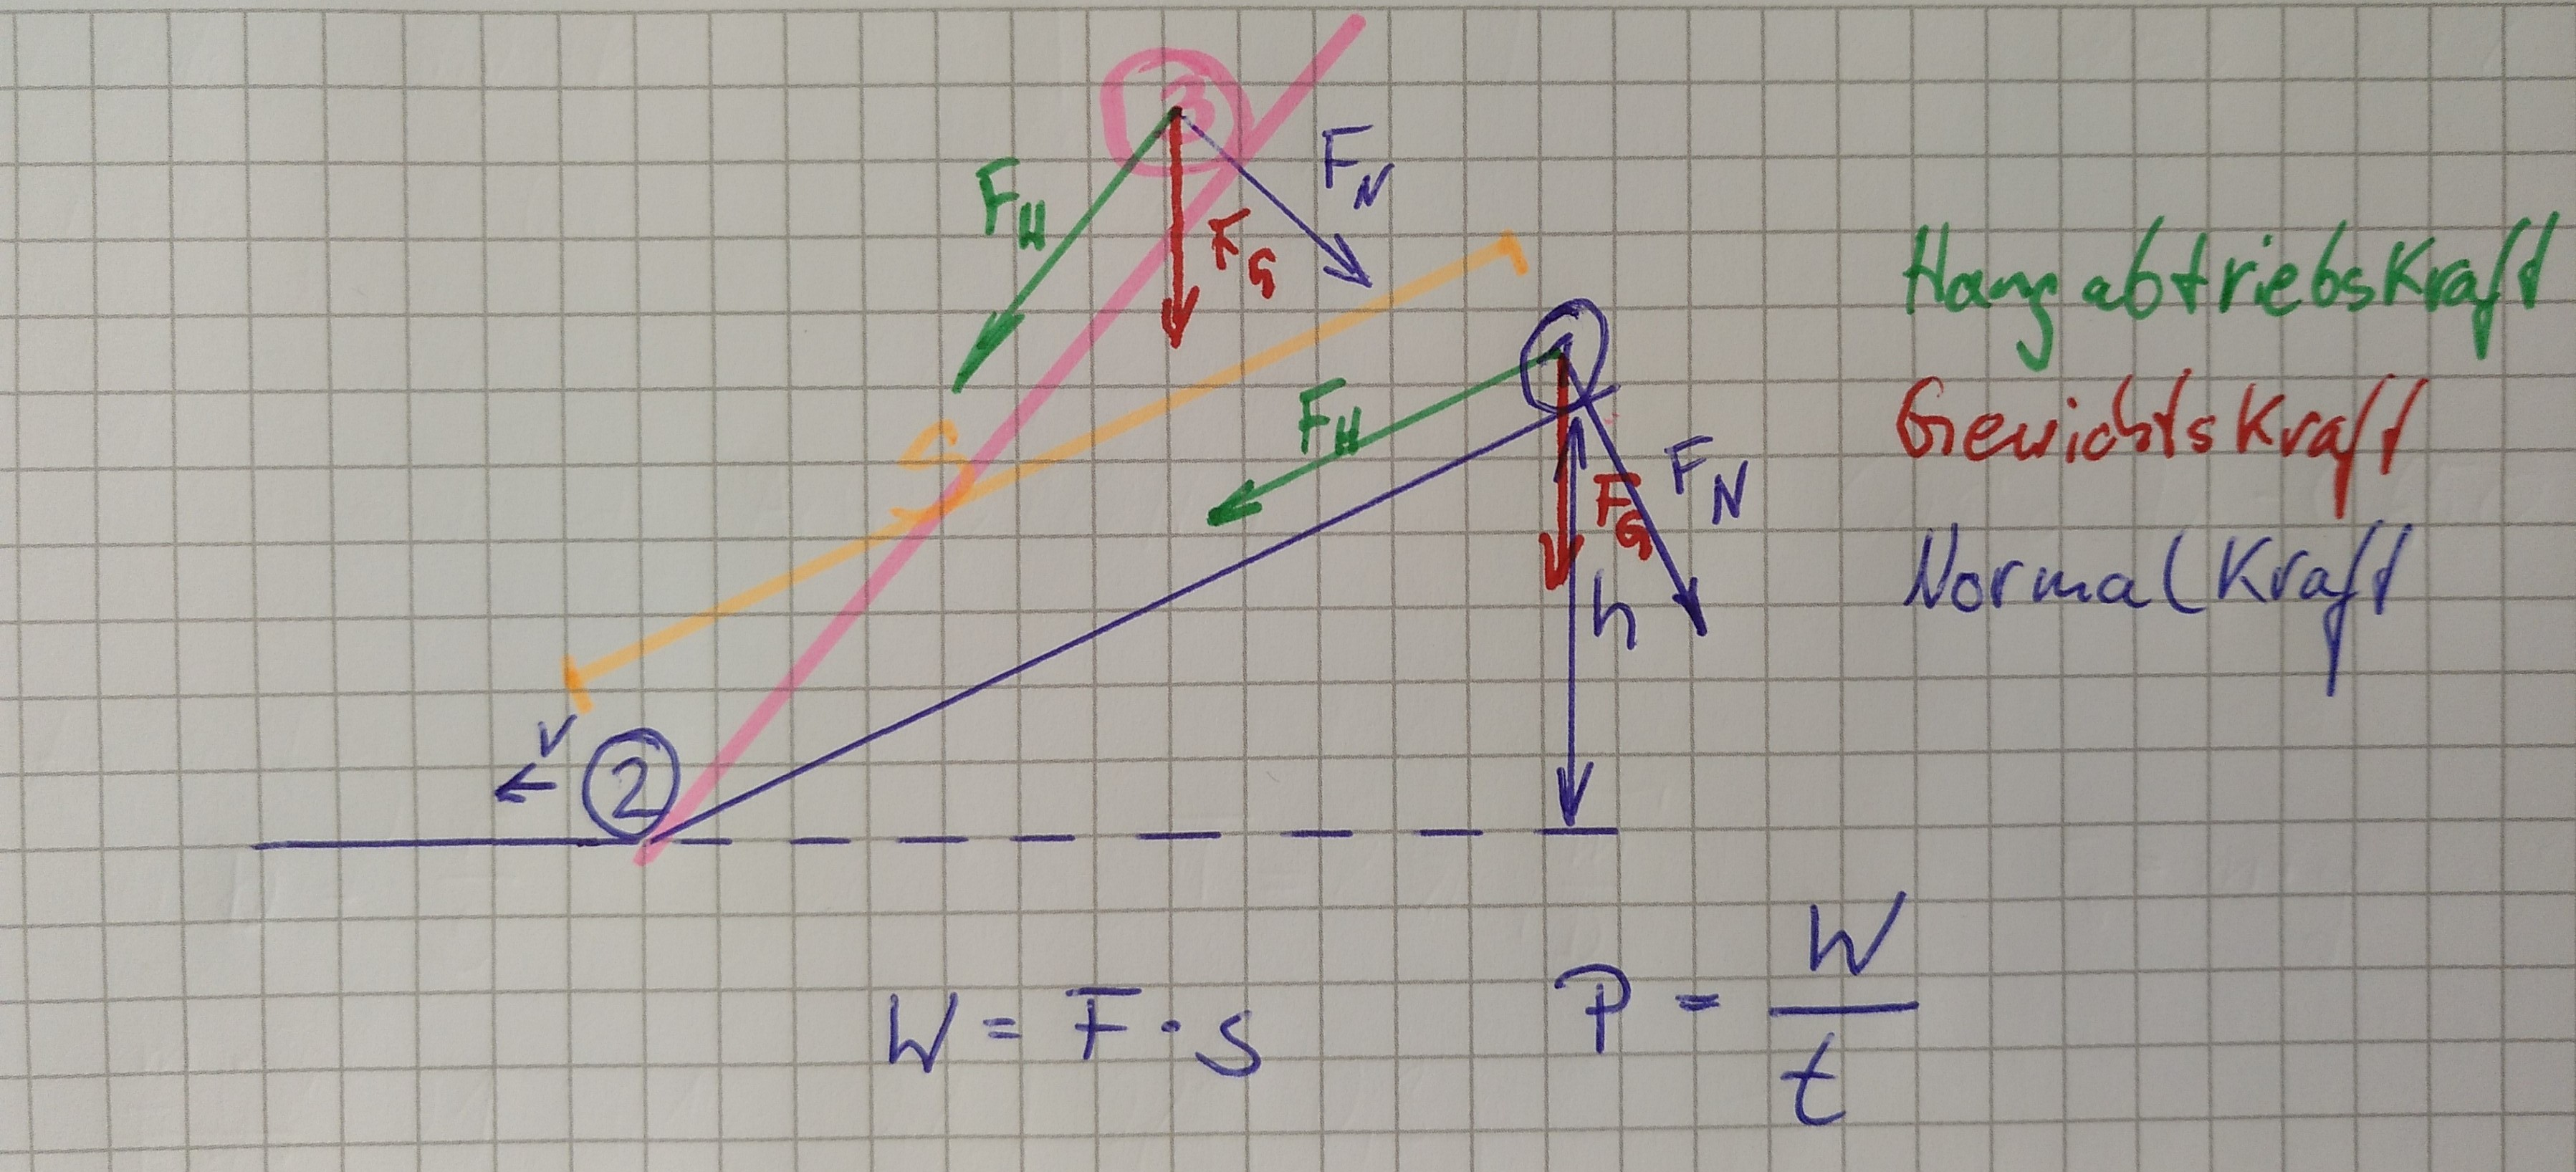
\includegraphics[width=0.75\textwidth]{Leistung}
	  \vspace{-3mm}
	  \caption{Potential an der schiefen Ebene}
   \end{figure}
}

\frame
{
  \frametitle{Feld}
\begin{block}{Beschreibung}
Ein "Feld" nennt man einen Bereich im Raum, in dem auf einen Körper eine Kraft wirkt. z.B. das Gravitationsfeld der Erde.
\end{block}
      \begin{figure}
	  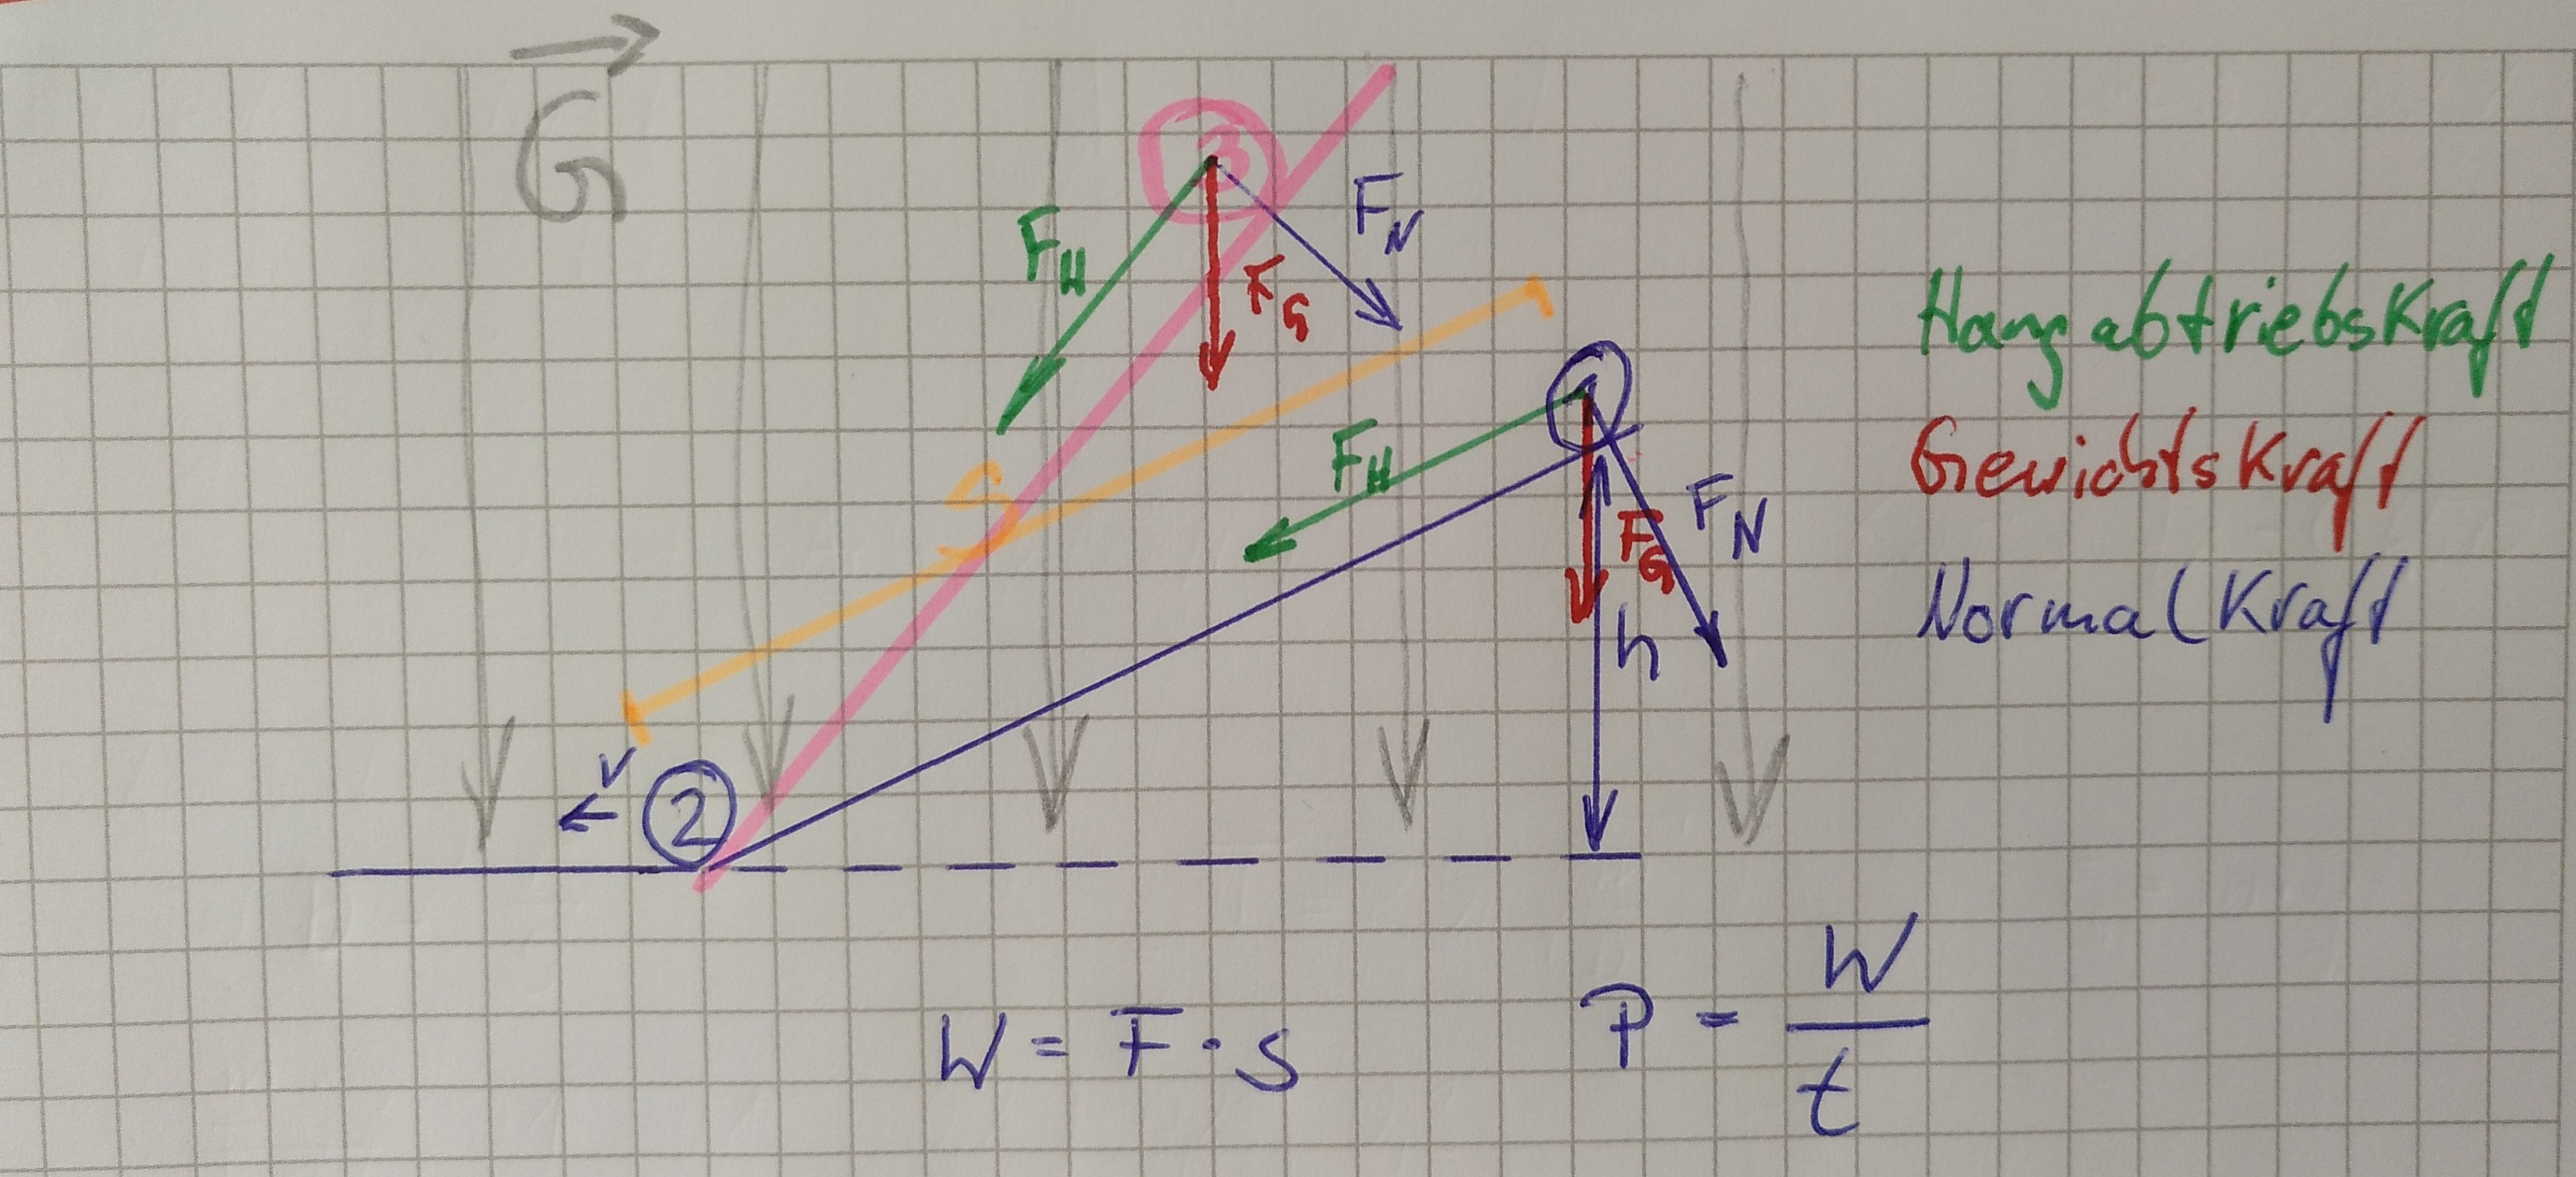
\includegraphics[width=0.8\textwidth]{Feld}
	  \vspace{-3mm}
	  \caption{Gravitationsfeld an der schiefen Ebene}
   \end{figure}
}
\end{document}
